\chapter{A motivation for studying fluid-structure interaction}
Fluid-structure interaction(FSI) is an interdiciplinary field, appearing in many applications. In nature, FSI forms the basis of many physical phenomia. A fish swimming utpstream,
generating thrust from the surrounding fluid by wave-like movements of its fin and body. Or a tree, bedning back and fourth due to strong winds of a storm passing by. Both examples are understandable, but points out two main instances of how FSI occur. When the fish swims, it deformes the fluid, altering the nearby flowfield. For the tree however, the swinging and bending is induced by the pressure of passing wind acting on the tree trunk and branches. Ultimatly, fluid-structure interaction occurs due to both initial effect of either fluid, structure or a combination.  \\

\newpage
Computational fluid-structure interaction (CFSI) has grown wast within engingeering in the recent years, and proved to be essential for design development and performance optimalizastion of many applications. Applications are, but not limited to biomedical computations such as heart valves and aneurisms(\cite{Torii2008}, \cite{Vierendeels2007}) inflation of parachutes \cite{Stein2001} ,Underwater explosions \cite{Kim2008} and wind turbines \cite{Hsu2012}.

Within aeronautics, CFSI have proven to be crucial for advances within flight characteristics and fuel economy. Due to a wide range of  wing materials and flow profiles to be studied, CFSI have made testing of proposed models possible, while saving expences regarding small and full-scale experiments. \newline

\begin{wrapfigure}{r}{0.5\textwidth}
  %\vspace{-10pt}
  \begin{center}
  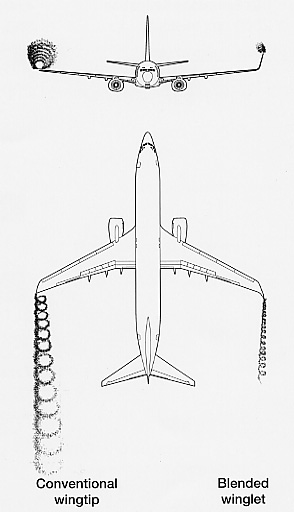
\includegraphics[scale=0.5]{./Fig/winglet.png}
  \end{center}
  %\vspace{-5pt}
  \caption{A comparison of shedding vortices from conventional wingtip, versious a winglet.}
 %\vspace{-5pt}
\end{wrapfigure}
 Winglet, a near vertical tip replacement for a conventional wingtip of an aircraft, have reduced  drag induced by wingtip vortices during flight. As a result, the overall fuel consumption of long-distance flights have been reduced by $\sim 5 \%$, which is why winglets can be observed within many airliners today.  Another consequence of installing wingelts is the recution of wingtip vortices, which in turn reduces trailing turbulence behind the aircraft.  The trailing turbulence can intervene with flight controls of aircraft passing through it, making  wingles an important safety feature for flight traffic. \\ \\ \\


Given the multidiciplinary nature  of FSI, significant developments within the field have occured within recent years.
Traditionally, fluid and structure mechanics have been considered separate scientific fields, hower the complex interaction There are several causes for ,
coupling of equations and nonlinearity

Even though FSI play an important role within many scientific apllications,

Computational stuff, why now, refer to computational power etc


Få med beregningsorienterte, to interdiciplinary. 